% Robert Schulze
% Matrikelnummer: 555625
% thesis for the pro seminar on artificial intelligence at TUC 2019

% to do:
% resolve all missing citations & references
% style front page
% make citations apalike

\documentclass[a4paper, 11pt]{report}

% include TUC logo
\usepackage{graphicx}
\usepackage{titling}
\author{Robert Schulze}
\title{Machine Music Generation: Using Neural Networks To Produce Metal Music}
\date{\today}


\usepackage{setspace}
\onehalfspacing

% set margins to 1 inch
\usepackage[margin=1in]{geometry}

% natbib for bibliography style
\usepackage{apalike}


% set font to TNR
\usepackage{mathptmx}
\usepackage[T1]{fontenc}

\begin{document}


\begin{titlepage}
    \begin{center}
        
\includegraphics[height=5cm]{tuc-gruen.png}
        
        \begin{large}
            \thetitle \\
            \theauthor \\
            \date{\today}  
            
        \end{large}
        
    \end{center}
\end{titlepage}

% use roman numbering for chapters
\renewcommand{\thechapter}{\Roman{chapter}}

\setcounter{page}{1} 

\tableofcontents

\chapter*{Abstract}
This paper introduces the Dadabots project and uses it as an example for the 
current status of research on audio synthesis using Artificial Neural 
Networks. Throughout the text, I am going to explore the SampleRNN architecture 
and explain Recurrent Neural Networks in a slightly broader fashion, as these 
are the underlying technologies of Dadabots. In the next step I am going to 
explain the reasons of the project’s authors to choose these specific 
technologies. In the conclusion of this text I counter the notion of ‘the death 
of creativity’ through artificial intelligence as I hope to provide a provide 
a perspective on how Artificial Neural Networks and Deep Learning can 
provide new ways of artistic expression.

\chapter{Introduction}
Dadabots is an ongoing experiment by Zack Zukowsky and CJ Carr, with the main 
aim of exploring modern advances in AI (‘Artificial Intelligence’) research on 
music synthesis in conjunction with popular music, namely Black Metal. They 
claim, that most training data used in this area of research focuses on 
classical music which pursues the ideal of the most harmonic composition. 
In contrast, modern music composition increasingly uses timbre manipulations as 
creative techniques over explorations of different 
tonalities\cite{zukowski2018generating}, thus training an 
ANN (‘Artificial Neural Network’) on this kind of data may yield very different 
results compared to more traditional approaches. \\
Moreover, the authors state that most research in the realm of music synthesis 
produces output in the symbolic domain only\cite{zukowski2018generating}. In this context this typically means 
the generation of midi notes which represent melodies and rhythms. Opposed to 
this, Carr and Zukowsky’s approach produces music on a sample-based approach, 
one sample at a time\cite{mehri2016samplernn}\cite{zukowski2018generating}.  \\
For this purpose the researchers adapted an ANN, SampleRNN, and used different 
albums by bands of the likes of Meshuggah and NOFX as Datasets. The results of 
this process are publicly available on 
Bandcamp\footnote{ https://dadabots.bandcamp.com/ } and in a 24/7 
Youtube\footnote{https://www.youtube.com/watch?v=CNNmBtNcccE } live 
stream and were first presented on the International Conference on Learning 
Representations (ICLR) in 2017. 

\chapter{SampleRNN}
SampleRNN is a \textit{Recurrent Neural Network} architecture that is specifically 
geared towards audio training data, i.e. speech and music, and the synthesis 
of such. The project was first presented at ICLR 2017 and is, according to 
Mehri et al. (2017) %revisit this citation -> apalike?
, “a novel model for unconditional audio generation 
based on generating one audio sample at a time”. \\
Synthesizing actual audio signals is a very recent development in the 
research on Neural Networks, since the actual computational cost for this 
task is very high. The authors put the average number of samples per word 
generated at a sample rate of 16 kHz (which, for example, is far below 
modern music production standards) at 6000\cite{mehri2016samplernn}. 
In prior approaches, this 
challenge would have been tackled with conversions of the raw audio 
beforehand (e.g. to spectrographs) to extract features which would then 
have been used as training data. The output then required further 
adjustment via DSP (‘Digital Signal Processing’) chains. \\
An additional challenge with this task is in the nature of audio data itself: 
in speech and music, dependencies between a sample (or a batch of them, as in 
a word or a musical phrase) and another one are often far apart from another. 
In orchestral music for example, composers use recurring themes that are 
used and varied throughout the length of a piece of music. To be able to learn 
these dependencies an ANN needs to be able to access data it learned much before 
the information which came immediately prior. In other words, the ANN needs to 
able to ‘remember’. RNNs (‘Recurrent Neural Networks’), unlike FNNs 
(Feedforward Neural Networks
\footnote{The term \textit{Feedforward Neural Networks}, 
also called \textit{Multilayer Perceptron} (MLP) describes a class of ANNs, 
which produce different output for each time step based on the the immediate 
information in the data stream. They do not use any feedback loops that allow 
information to persist and alter the state of nodes based on a batch of information.
\cite[p. 164]{goodfellow2016deep}}), 
have the ability to use these information. Aside 
from processing audio data, other applications of RNNs include Emotion Recognition
\cite{ebrahimi2015recurrent}, 
Gesture Recognition\cite[]{murakami1991gesture}, and Video Translation\cite{venugopalan2014translating}.  \\

\section{Recurrent Neural Networks}
RNNs enhance the concept of FNNs with Feedback Loops, that allow information to 
persist in a node. For this reason RNNs are able to learn from sequential data, 
such as a sequence of samples. \\
One of the main features of this architecture is the ability to \textit{share parameters} 
between elements of a single model: This for example applies in a single node, 
that keeps parameters it has learned in a prior timestep and applies those later. 
But also parameters may be exchanged between nodes. \\
Parameter Sharing has two advantages: it reduces the overall computational cost 
of training a model, because the overall number of parameters that has to be 
learned is reduced, compared to learning these anew with every timestep. Also, 
it enables the network to process data sequences of varying lengths
\cite[pp.367]{goodfellow2016deep}: the number 
of parameters to be learned grows with the length of the sequence. Since 
parameters persist in the network it becomes independent from the number of 
timesteps necessary to learn a sequence. Usually, this process is schematically 
visualized using an \textit{unrolled graph} as shown in figure \ref{fig1:unrolledgraph}.
% unrolled graph picture environment
\begin{figure}[h!]
    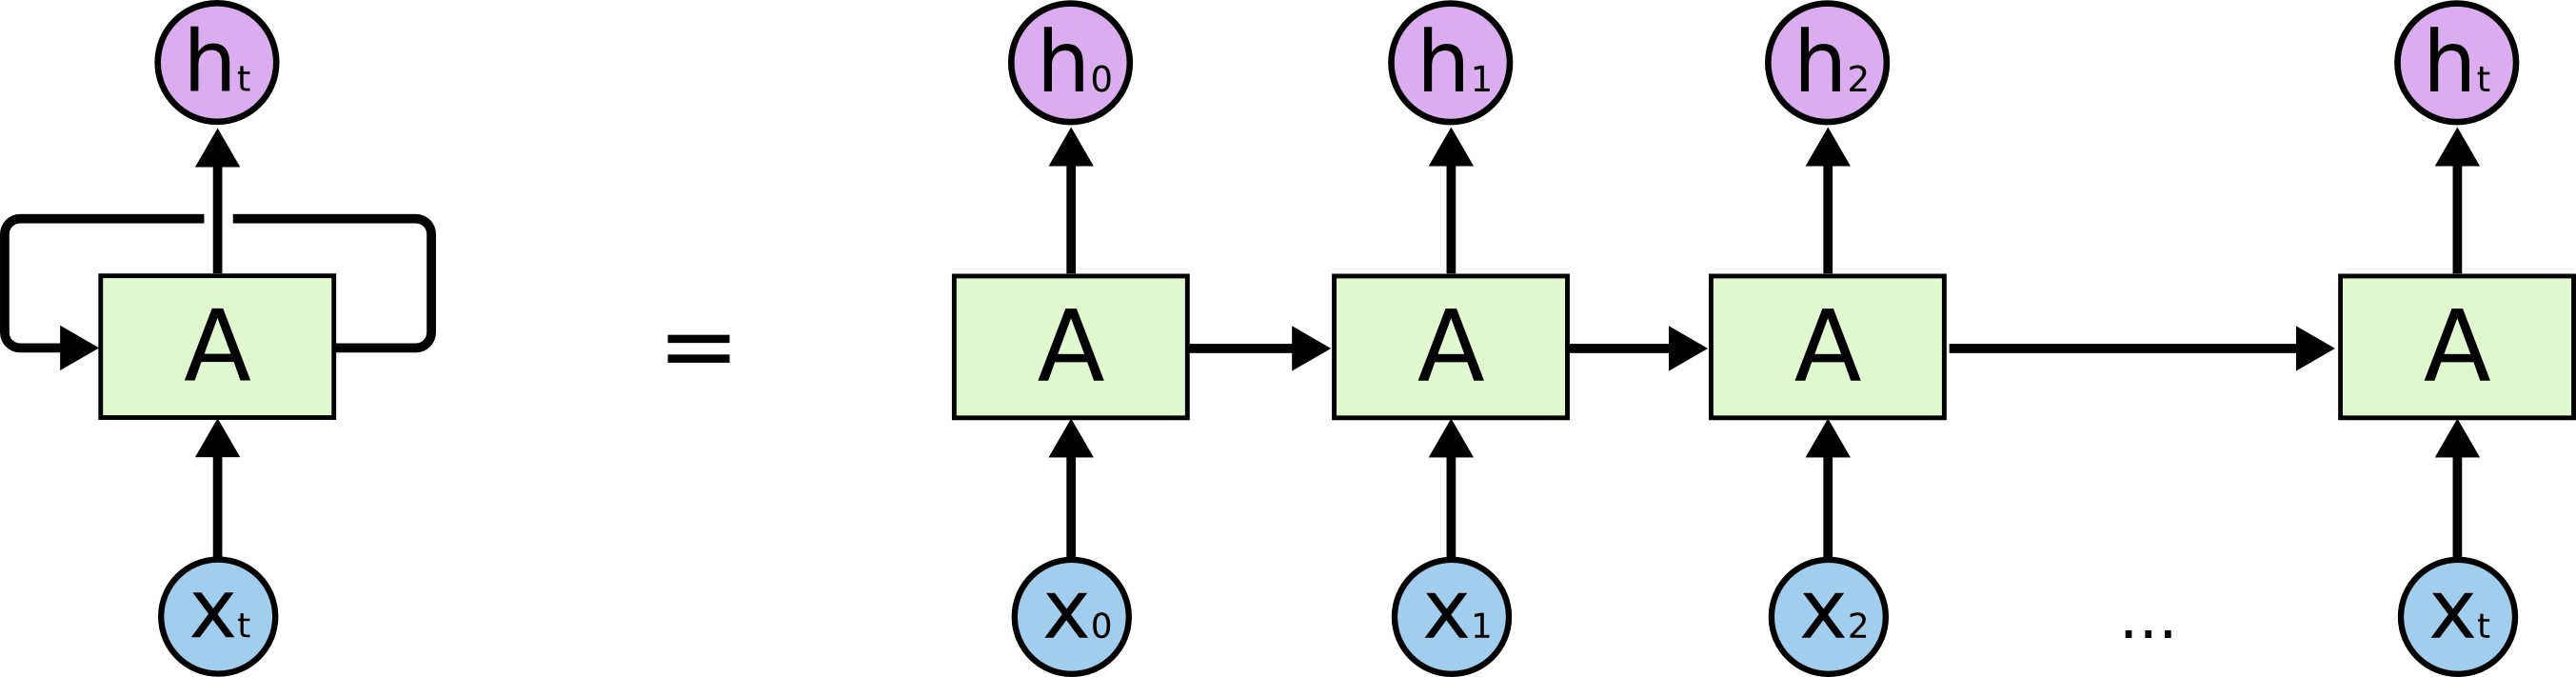
\includegraphics[width=\linewidth]{rnn_unrolled.png}
    \caption{This image shows the feedback loop on the left side and an unrolled 
    version on the right: input is taken with every timestep from the training data 
    as well as from prior timestep.
    source: http://colah.github.io/posts/2015-08-Understanding-LSTMs/
    }
    \label{fig1:unrolledgraph}
\end{figure}

\section{Multi-Tier Structure}
SampleRNN furthers the idea of Parameter Sharing by introducing tiers which 
consist of recurrent units (except the lowest tier, which consists of MLPs) and 
are organized in a hierarchical structure. Parameters are shared within the 
tiers itself as well as passed down to lower ones. The tiers operate at different 
clock-rates, with the sizes of sequences (Mehri et al. call these sequences Frames) 
processed in each tier gradually decreasing as the output of each tier is passed 
as a single conditioning vector down the hierarchy. This is possible through 
upsampling\footnote{Upsampling denotes the process of increasing the actual number of 
samples in a sequence via interpolation. 
}
in-between tiers, with the lowest operating at single-sample level, 
as shown in figure \ref{fig2:samplernn}. Consequently, the lowest tier also 
outputs single samples. \\
An advantage of this approach compared to models which operate on sample-level 
only is the reduced amount of computations necessary and therefore a faster and 
more efficient training process. Furthermore it betters the model’s ability to 
learn non sample-level dependencies. \\
For their experiment, Mehri et al. used both a two-tier and a three-tier model.
\begin{figure}[h!]
    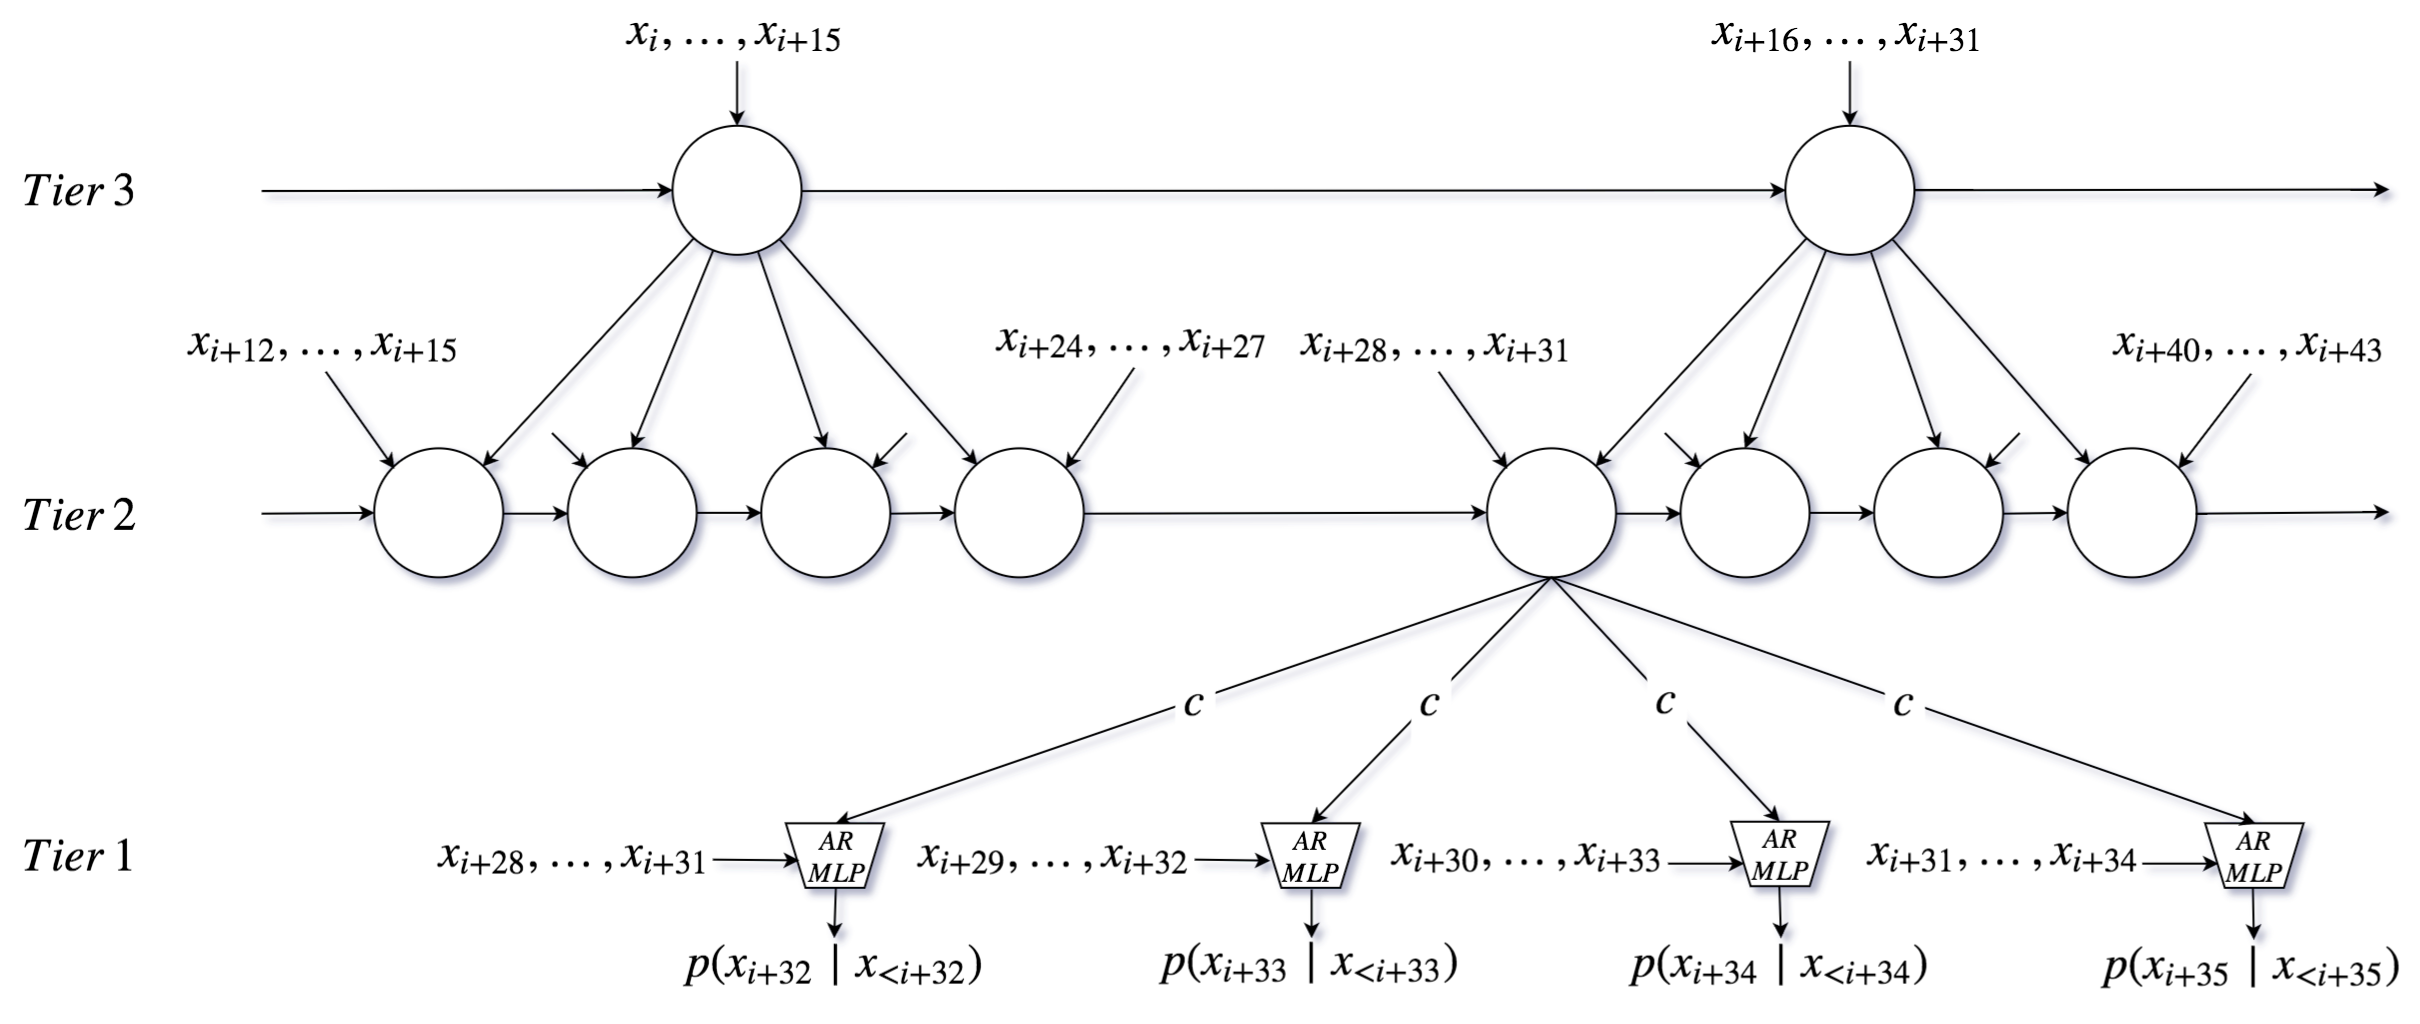
\includegraphics[width=\linewidth]{samplernn.png}
    \caption{Computational Graph for the 3-Tier SampleRNN model. The decreasing 
    frame sizes of input are visible in the number of timesteps of the parameters. 
    Recurrent units are represented as circles while MLPs are rectangular. Tiers 
    2 and 3 are supplied with training data directly while tiers 1 and 2 are 
    passed parameters from the respective higher tier.
    source: Mehri, Soroush, et al. "SampleRNN: An unconditional end-to-end 
    neural audio generation model." arXiv preprint arXiv:1612.07837 (2016).
    }
    \label{fig2:samplernn}
\end{figure}
However, practice has shown that the output quality of standard RNNs degrades\footnote{
    Although RNNs should be perfectly capable to retain information for a very long time 
    in theory, experiments have shown, that their parameters tend to 0 or infinity when 
    trained on real-world data. This is called Vanishing Gradient Problem: the values 
    used to update the weights might be too small to change the values and thus prevent 
    the network from training effectively. This is especially problematic with the 
    limited precision of floating-point values used which are used for the calculations, 
    Not as common but at least as challenging are Exploding Grades which occur when 
    grades become too big and the weights then tend towards infinity\cite[p.286, 
    pp.396]{goodfellow2016deep}. 
} 
with the growth of the length of the sequences used in training. As a consequence, 
baseline recurrent architecture was complemented with \textit{Long Short Term Memory} 
(LSTM) Modules, which are able to retain parameters for a much longer time, and 
also to learn, when the right time to forget those parameters is. This is possible 
because of the introduction of gates to those cells: An input and a forget gate 
allow the unit to compute if it is necessary to accumulate information of former 
timesteps, while the output gate allows to hold back output for the next timestep. \\
The concept of LSTMs has been introduced by Hochreiter and Schmidhuber (1997) and 
is used in many variations now. One of the updates made to LSTMs are \textit{Gated Recurrent 
Units} (GRUs). Here, input and forget gate are combined in one single gate.

\section{The Traning Process}
For comparability, the authors trained both a two- and a three-tier structure 
on three different data sets related to speech and music, respectively: the 
first one, \textit{Blizzard}, contains 315 hours of recordings\footnote{the 
authors used only 20.5 hours thereof for the experiment
} 
of a female english-speaking 
actor, the second, \textit{Onomatopeia}, contains 3.5 hours of vocal sounds (e.g. grunting, 
shouting, coughing), and finally a \textit{Music} data set comprised of 32 Beethoven sonatas 
totalling 10 hours. All data sets were used at 16 kHz sample rate and 16 bit depth 
and split up to 8 seconds long sequences\footnote{with the exception of the Onomatopeia set, 
which contains only samples of 1 to 11 seconds length}. 
The training took about one Week on a single GPU per Model and Data Set. Recurrent Units were 
implemented both as LSTMs and GRUs, while Mehri et al (2017) found the results of the latter 
being marginally better than those of the former. 

\section{Qualification, Reception, And Other Approaches}
For comparison the training with exactly the same data was also performed on a 
baseline RNN model as well as a re-implementation of \textit{WaveNet}\footnote{
    WaveNet is a neural architecture proposed by DeepMind with the same purpose 
    as SampleRNN: generating audio signals. However, unlike SampleRNN, it uses 
    convolutional layers which are not able to operate at different clock rates 
    but instead operate at sample level only\cite{van2016wavenet}
}\footnote{
    The WaveNet re-implementation, however, differs from the original one due 
    to the lack of information on hyperparameters and the lack of computational 
    resources.
}. The resulting 
output of 2-Tier and 3-Tier models as well as the reference models was evaluated 
by both computing the NLL (‘Negative Logarithmic Likelihood’)\footnote{
    The NLL is commonly used as the loss function to compute accuracy of the 
    output of a Neural Network. The lower the value, the higher the accuracy. 
    In generative Models this value is often represented in bits, here in bits 
    per sample.
} and human evaluation\footnote{
    Precisely, the authors conducted AB-Preference test with random samples 
    generated from the training on the Blizzard and Music data sets.
}. \\
The results of both evaluation methods overwhelmingly favoured the SampleRNN 
architectures: The 3-Tier model scored the lowest NLL values for the Onomatopeia 
and Blizzard data sets, with the 2-Tier model having the best result for the 
Music data set\footnote{Interestingly, the Music data set showed the lowest 
NLL values across all four models while the Onomatopeia set had the highest. 
This suggests, that piano music works far better as training data for sound 
synthesis than speech sounds.  
}. \\
Likewise, the 3-Tier model was preferred by listeners over the results of all other 
models for the audio resulting from the training on speech, while the 2-Tier model 
scored best results with regards to the training on music. \\
These results show clearly, that SampleRNN marks a step forward for the field of 
neural audio generation. A further indicator for the quality of the architecture 
are the reduced training times and the smaller computational cost compared to 
WaveNet. These two are the main reasons, Carr and Zukowsky chose SampleRNN to 
conduct their experiments on Metal Music. \\


\chapter{The Results of Dadabots}
As already mentioned, Dadabots is trained on a single album at a time, which 
is preprocessed by splitting up the audio data into 8-second long sequences and 
then training the model for about 50.000-80.000 iterations at a time, which 
roughly equals 3 days of total training time on a single GPU per album. The 
architecture used is the 2-Tier variant of SampleRNN, as it has shown the best 
results for music-related data. The Training is stopped at checkpoints when 10 
30-second samples are generated and compressed to wav.. The authors observed, 
that early in the training the generation of textures dominated, whereas later 
in the training process “[...] riffs and sectional transitions [...]” (Carr
and Zukowsky, 2017) were 
produced. After a certain time the model starts to produce white noise only 
and the authors restarted the training.

\section{Results}
The aim was to reproduce the training data as good as possible. While the 
results were not simple copies of the training data, both quality of the sound 
as well as the similarity between input and output were surprising and suggest, 
that training ANNs on non-classical music might be something research should 
turn to more. \\
The authors note, that they were particularly delighted by the variations 
SampleRNN introduced to the music. They note, that: “Solo vocalists become a 
lush choir of ghostly voices, rock bands become crunchy cubist-jazz, and cross-
breeds of multiple recordings become a surrealist chimera of sound.“\cite[p.3]{zukowski2018generating} 
The abrupt 
rhythmic changes and radical tonal colour were closer to Math Rock, since those 
do not exist in Black Metal. Finally, they suggest that Artists might further 
explore these new aesthetics that neural audio generation introduces.

\chapter{Discussion}
As outlined, projects such as SampleRNN and WaveNet mark an important stepping 
stone in artificial audio synthesis, since they make the generation of actual 
audio data, as opposed to its symbolic representation, possible for the first 
time. The Dadabots approach has shown, that non-conventional training data may 
yield unexpected and interesting results, which introduce new aesthetics and 
deviate from simply replicating the training data. \\
These findings contrast the discourse about the ‘End of Creativity’\cite{chenne2018}
because 
of the the standardization of taste in music, or art in a broader sense, via 
prediction algorithms\footnote{
    These predictions are the result of the analysis of massive data lots 
    through ANNs. 
} such as those of Youtube, Facebook, or Spotify. While I 
agree, that the predictions used by these platforms change the way music is 
monetized in that they favor music published my major labels with substantial 
marketing budgets\cite{lindvall2009}, ANNs may be used in new creative ways 
as shown above. \\
Future work should focus on creating applications that allow for simple 
adjustment of parameters of the model and implementation of built-in DSP 
methods, so that these models may be used similar to a software instrument. 
Also further research as to the optimization of the training process has to 
be conducted, since most people are not able to deploy high-scale computational 
infrastructures and industry-standard GPUs, so will not be able to train a 
model in a feasible amount of time. These steps would allow for a much broader 
application of neural audio synthesis.   



\bibliographystyle{apalike}
\bibliography{biblio}


\end{document}